\section{Metodo di Newton}
\label{sec:metodoDiNewton}

\begin{exercise}
Implementare il metodo di newton ed applicarlo alla funzione \emph{singleZero},
con innesco iniziale $x_{0} = 7$, una tollerenza assoluta e relativa
$tol_{X} = rTol_{X} = 10^{-14}$ ed un numero massimo di iterazioni
$i_{max} = 10^{2}$.
\end{exercise}
Per l'implementazione del codice vedere \nameref{sec:newtonIterativeMethod}.
\begin{lstlisting}
octave:112> [x, i, ascisse] = newtonMethod('singleZero', 'singleZeroDerivative',7, 1e2, 1e-14, 1e-14) 
x =  3.40512483795333e+00
i =  5.00000000000000e+00
ascisse = [too long to report here]
octave:113> xSingleZero = min(ascisse)-1:0.1:max(ascisse)+1
octave:114> ySingleZero = invokeDelegate('singleZero', xSingleZero)
octave:115> [prepX, prepY] = prepareForPlottingMethodSegments(ascisse, 'invokeDelegate', 'singleZero')
octave:116> plot(xSingleZero, ySingleZero, "c", ascisse, invokeDelegate('singleZero', ascisse), "b+", prepX, prepY, "r")
octave:117> grid
octave:118> print 'newtonPlotOutput.tex' '-dTex' '-S800, 600'
\end{lstlisting}
Si raggiunge la tolleranza richiesta in 5 passi. Questo l'output del comando
\emph{octave:118}:
\begin{center}
% GNUPLOT: LaTeX picture with Postscript
\begingroup
  \makeatletter
  \providecommand\color[2][]{%
    \GenericError{(gnuplot) \space\space\space\@spaces}{%
      Package color not loaded in conjunction with
      terminal option `colourtext'%
    }{See the gnuplot documentation for explanation.%
    }{Either use 'blacktext' in gnuplot or load the package
      color.sty in LaTeX.}%
    \renewcommand\color[2][]{}%
  }%
  \providecommand\includegraphics[2][]{%
    \GenericError{(gnuplot) \space\space\space\@spaces}{%
      Package graphicx or graphics not loaded%
    }{See the gnuplot documentation for explanation.%
    }{The gnuplot epslatex terminal needs graphicx.sty or graphics.sty.}%
    \renewcommand\includegraphics[2][]{}%
  }%
  \providecommand\rotatebox[2]{#2}%
  \@ifundefined{ifGPcolor}{%
    \newif\ifGPcolor
    \GPcolortrue
  }{}%
  \@ifundefined{ifGPblacktext}{%
    \newif\ifGPblacktext
    \GPblacktexttrue
  }{}%
  % define a \g@addto@macro without @ in the name:
  \let\gplgaddtomacro\g@addto@macro
  % define empty templates for all commands taking text:
  \gdef\gplbacktext{}%
  \gdef\gplfronttext{}%
  \makeatother
  \ifGPblacktext
    % no textcolor at all
    \def\colorrgb#1{}%
    \def\colorgray#1{}%
  \else
    % gray or color?
    \ifGPcolor
      \def\colorrgb#1{\color[rgb]{#1}}%
      \def\colorgray#1{\color[gray]{#1}}%
      \expandafter\def\csname LTw\endcsname{\color{white}}%
      \expandafter\def\csname LTb\endcsname{\color{black}}%
      \expandafter\def\csname LTa\endcsname{\color{black}}%
      \expandafter\def\csname LT0\endcsname{\color[rgb]{1,0,0}}%
      \expandafter\def\csname LT1\endcsname{\color[rgb]{0,1,0}}%
      \expandafter\def\csname LT2\endcsname{\color[rgb]{0,0,1}}%
      \expandafter\def\csname LT3\endcsname{\color[rgb]{1,0,1}}%
      \expandafter\def\csname LT4\endcsname{\color[rgb]{0,1,1}}%
      \expandafter\def\csname LT5\endcsname{\color[rgb]{1,1,0}}%
      \expandafter\def\csname LT6\endcsname{\color[rgb]{0,0,0}}%
      \expandafter\def\csname LT7\endcsname{\color[rgb]{1,0.3,0}}%
      \expandafter\def\csname LT8\endcsname{\color[rgb]{0.5,0.5,0.5}}%
    \else
      % gray
      \def\colorrgb#1{\color{black}}%
      \def\colorgray#1{\color[gray]{#1}}%
      \expandafter\def\csname LTw\endcsname{\color{white}}%
      \expandafter\def\csname LTb\endcsname{\color{black}}%
      \expandafter\def\csname LTa\endcsname{\color{black}}%
      \expandafter\def\csname LT0\endcsname{\color{black}}%
      \expandafter\def\csname LT1\endcsname{\color{black}}%
      \expandafter\def\csname LT2\endcsname{\color{black}}%
      \expandafter\def\csname LT3\endcsname{\color{black}}%
      \expandafter\def\csname LT4\endcsname{\color{black}}%
      \expandafter\def\csname LT5\endcsname{\color{black}}%
      \expandafter\def\csname LT6\endcsname{\color{black}}%
      \expandafter\def\csname LT7\endcsname{\color{black}}%
      \expandafter\def\csname LT8\endcsname{\color{black}}%
    \fi
  \fi
  \setlength{\unitlength}{0.0500bp}%
  \begin{picture}(7680.00,5760.00)%
    \gplgaddtomacro\gplbacktext{%
      \colorrgb{0.00,0.00,0.00}%
      \put(866,634){\makebox(0,0)[r]{\strut{}-10}}%
      \colorrgb{0.00,0.00,0.00}%
      \put(866,1304){\makebox(0,0)[r]{\strut{}0}}%
      \colorrgb{0.00,0.00,0.00}%
      \put(866,1975){\makebox(0,0)[r]{\strut{}10}}%
      \colorrgb{0.00,0.00,0.00}%
      \put(866,2645){\makebox(0,0)[r]{\strut{}20}}%
      \colorrgb{0.00,0.00,0.00}%
      \put(866,3316){\makebox(0,0)[r]{\strut{}30}}%
      \colorrgb{0.00,0.00,0.00}%
      \put(866,3986){\makebox(0,0)[r]{\strut{}40}}%
      \colorrgb{0.00,0.00,0.00}%
      \put(866,4657){\makebox(0,0)[r]{\strut{}50}}%
      \colorrgb{0.00,0.00,0.00}%
      \put(866,5327){\makebox(0,0)[r]{\strut{}60}}%
      \colorrgb{0.00,0.00,0.00}%
      \put(998,414){\makebox(0,0){\strut{}2}}%
      \colorrgb{0.00,0.00,0.00}%
      \put(1990,414){\makebox(0,0){\strut{}3}}%
      \colorrgb{0.00,0.00,0.00}%
      \put(2982,414){\makebox(0,0){\strut{}4}}%
      \colorrgb{0.00,0.00,0.00}%
      \put(3974,414){\makebox(0,0){\strut{}5}}%
      \colorrgb{0.00,0.00,0.00}%
      \put(4966,414){\makebox(0,0){\strut{}6}}%
      \colorrgb{0.00,0.00,0.00}%
      \put(5958,414){\makebox(0,0){\strut{}7}}%
      \colorrgb{0.00,0.00,0.00}%
      \put(6950,414){\makebox(0,0){\strut{}8}}%
    }%
    \gplgaddtomacro\gplfronttext{%
    }%
    \gplbacktext
    \put(0,0){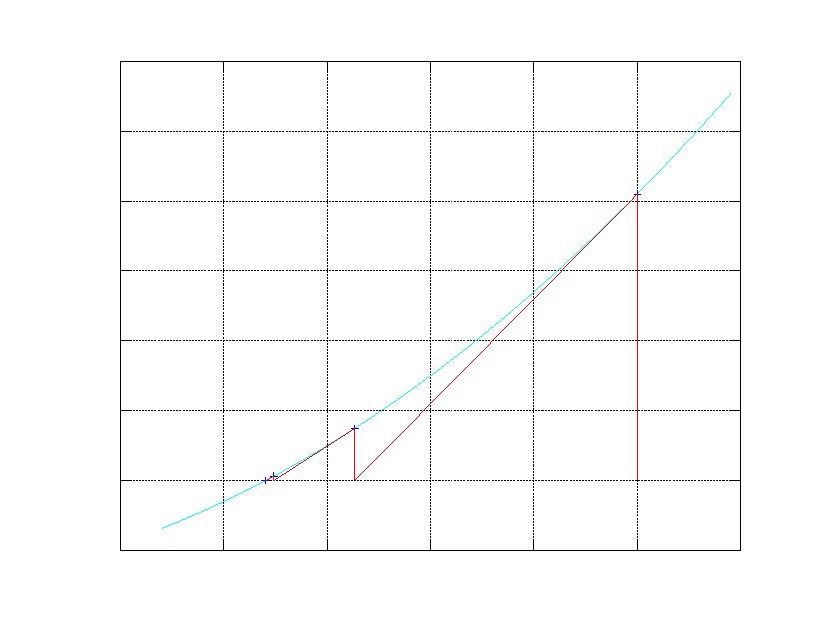
\includegraphics{RadiciEquazione/newton/newtonPlotOutput}}%
    \gplfronttext
  \end{picture}%
\endgroup

\end{center}

\begin{exercise}
Implementare il metodo di newton ed applicarlo alla funzione \emph{functionWithNoRealZero},
con innesco iniziale $x_{0} = 2.5$, una tollerenza assoluta e relativa
$tol_{X} = rTol_{X} = 10^{-14}$ ed un numero massimo di iterazioni
$i_{max} = 7$.
\end{exercise}
Per l'implementazione del codice vedere \nameref{sec:newtonIterativeMethod}.
\begin{lstlisting}
octave:112> [x, i, ascisse] = newtonMethod('functionWithNoRealZero','functionWithNoRealZeroDerivative', 2.5, 7, 1e-14, 1e-14)
Il metodo non converge.
x = -3.18786023393994e+00
i =  7.00000000000000e+00
ascisse = [too long to report here]
octave:113> xNoZero = min(ascisse)-1:0.1:max(ascisse)+1
octave:114> yNoZero = invokeDelegate('functionWithNoRealZero', xNoZero)
octave:115> [prepX, prepY] = prepareForPlottingMethodSegments(ascisse, 'invokeDelegate', 'functionWithNoRealZero')
octave:116> plot(xNoZero, yNoZero, "c", ascisse,invokeDelegate('functionWithNoRealZero', ascisse), "b+", prepX, prepY, "r")
octave:117> grid
octave:118> print 'newtonNoZeroPlotOutput.tex' '-dTex' '-S800, 600'
\end{lstlisting}
Non si raggiunge la convergenza, infatti vengono fatti il massimo possibile
dei passi fissati dal parametro $i_{max}$. Questo l'output del comando \emph{octave:118}:
\begin{center}
% GNUPLOT: LaTeX picture with Postscript
\begingroup
  \makeatletter
  \providecommand\color[2][]{%
    \GenericError{(gnuplot) \space\space\space\@spaces}{%
      Package color not loaded in conjunction with
      terminal option `colourtext'%
    }{See the gnuplot documentation for explanation.%
    }{Either use 'blacktext' in gnuplot or load the package
      color.sty in LaTeX.}%
    \renewcommand\color[2][]{}%
  }%
  \providecommand\includegraphics[2][]{%
    \GenericError{(gnuplot) \space\space\space\@spaces}{%
      Package graphicx or graphics not loaded%
    }{See the gnuplot documentation for explanation.%
    }{The gnuplot epslatex terminal needs graphicx.sty or graphics.sty.}%
    \renewcommand\includegraphics[2][]{}%
  }%
  \providecommand\rotatebox[2]{#2}%
  \@ifundefined{ifGPcolor}{%
    \newif\ifGPcolor
    \GPcolortrue
  }{}%
  \@ifundefined{ifGPblacktext}{%
    \newif\ifGPblacktext
    \GPblacktexttrue
  }{}%
  % define a \g@addto@macro without @ in the name:
  \let\gplgaddtomacro\g@addto@macro
  % define empty templates for all commands taking text:
  \gdef\gplbacktext{}%
  \gdef\gplfronttext{}%
  \makeatother
  \ifGPblacktext
    % no textcolor at all
    \def\colorrgb#1{}%
    \def\colorgray#1{}%
  \else
    % gray or color?
    \ifGPcolor
      \def\colorrgb#1{\color[rgb]{#1}}%
      \def\colorgray#1{\color[gray]{#1}}%
      \expandafter\def\csname LTw\endcsname{\color{white}}%
      \expandafter\def\csname LTb\endcsname{\color{black}}%
      \expandafter\def\csname LTa\endcsname{\color{black}}%
      \expandafter\def\csname LT0\endcsname{\color[rgb]{1,0,0}}%
      \expandafter\def\csname LT1\endcsname{\color[rgb]{0,1,0}}%
      \expandafter\def\csname LT2\endcsname{\color[rgb]{0,0,1}}%
      \expandafter\def\csname LT3\endcsname{\color[rgb]{1,0,1}}%
      \expandafter\def\csname LT4\endcsname{\color[rgb]{0,1,1}}%
      \expandafter\def\csname LT5\endcsname{\color[rgb]{1,1,0}}%
      \expandafter\def\csname LT6\endcsname{\color[rgb]{0,0,0}}%
      \expandafter\def\csname LT7\endcsname{\color[rgb]{1,0.3,0}}%
      \expandafter\def\csname LT8\endcsname{\color[rgb]{0.5,0.5,0.5}}%
    \else
      % gray
      \def\colorrgb#1{\color{black}}%
      \def\colorgray#1{\color[gray]{#1}}%
      \expandafter\def\csname LTw\endcsname{\color{white}}%
      \expandafter\def\csname LTb\endcsname{\color{black}}%
      \expandafter\def\csname LTa\endcsname{\color{black}}%
      \expandafter\def\csname LT0\endcsname{\color{black}}%
      \expandafter\def\csname LT1\endcsname{\color{black}}%
      \expandafter\def\csname LT2\endcsname{\color{black}}%
      \expandafter\def\csname LT3\endcsname{\color{black}}%
      \expandafter\def\csname LT4\endcsname{\color{black}}%
      \expandafter\def\csname LT5\endcsname{\color{black}}%
      \expandafter\def\csname LT6\endcsname{\color{black}}%
      \expandafter\def\csname LT7\endcsname{\color{black}}%
      \expandafter\def\csname LT8\endcsname{\color{black}}%
    \fi
  \fi
  \setlength{\unitlength}{0.0500bp}%
  \begin{picture}(7680.00,5760.00)%
    \gplgaddtomacro\gplbacktext{%
      \colorrgb{0.00,0.00,0.00}%
      \put(866,634){\makebox(0,0)[r]{\strut{}0}}%
      \colorrgb{0.00,0.00,0.00}%
      \put(866,1807){\makebox(0,0)[r]{\strut{}5}}%
      \colorrgb{0.00,0.00,0.00}%
      \put(866,2981){\makebox(0,0)[r]{\strut{}10}}%
      \colorrgb{0.00,0.00,0.00}%
      \put(866,4154){\makebox(0,0)[r]{\strut{}15}}%
      \colorrgb{0.00,0.00,0.00}%
      \put(866,5327){\makebox(0,0)[r]{\strut{}20}}%
      \colorrgb{0.00,0.00,0.00}%
      \put(998,414){\makebox(0,0){\strut{}-6}}%
      \colorrgb{0.00,0.00,0.00}%
      \put(2188,414){\makebox(0,0){\strut{}-4}}%
      \colorrgb{0.00,0.00,0.00}%
      \put(3379,414){\makebox(0,0){\strut{}-2}}%
      \colorrgb{0.00,0.00,0.00}%
      \put(4569,414){\makebox(0,0){\strut{}0}}%
      \colorrgb{0.00,0.00,0.00}%
      \put(5760,414){\makebox(0,0){\strut{}2}}%
      \colorrgb{0.00,0.00,0.00}%
      \put(6950,414){\makebox(0,0){\strut{}4}}%
    }%
    \gplgaddtomacro\gplfronttext{%
    }%
    \gplbacktext
    \put(0,0){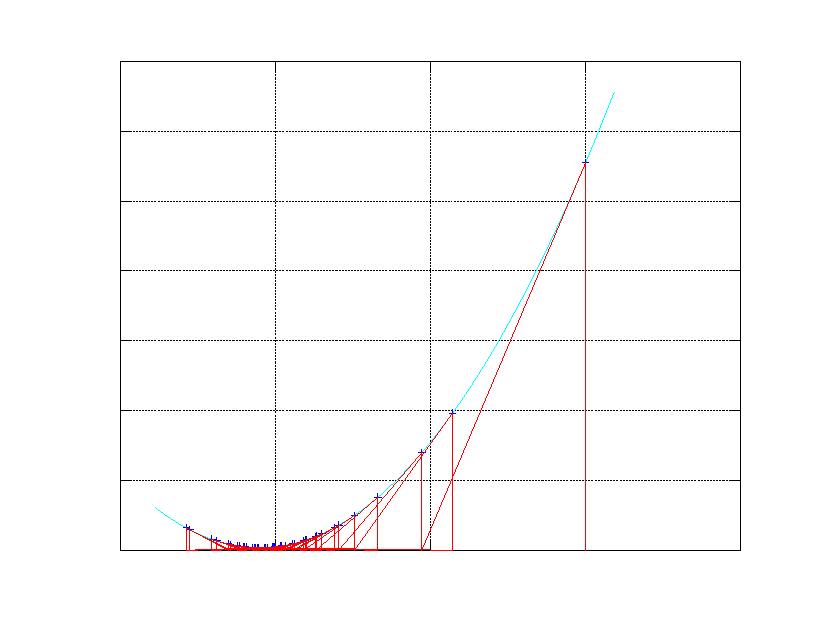
\includegraphics{RadiciEquazione/newton/newtonNoZeroPlotOutput}}%
    \gplfronttext
  \end{picture}%
\endgroup

\end{center}

\begin{exercise}[2.4]
Per il testo dell'esercizio consultare il libro di testo.
\end{exercise}
Per l'implementazione del codice vedere \nameref{sec:newtonIterativeMethod}.

Nel primo caso studio il punto di innesco $x_{0} = 10$:
\begin{lstlisting}
octave:112> [x, i, ascisse] = newtonMethod('functionNewtonRecursion','functionNewtonRecursionDerivative', 10, 5e1, 1e-14, 1e-14)
x =  2.23606797749979e+00
i =  9.00000000000000e+00
ascisse = [too long to report here]
octave:113> xNoZero = min(ascisse)-1:0.1:max(ascisse)+1
octave:114> yNoZero = invokeDelegate('functionNewtonRecursion', xNoZero)
octave:115> [prepX, prepY] = prepareForPlottingMethodSegments(ascisse, 'invokeDelegate', 'functionNewtonRecursion')
octave:116> plot(xNoZero, yNoZero, "c", ascisse,invokeDelegate('functionNewtonRecursion', ascisse), "b+", prepX, prepY, "r")
octave:117> grid
octave:118> print 'newtonRecursivePlotOutput.tex' '-dTex' '-S800, 600'
\end{lstlisting}
Si raggiunge la convergenza con 9 passi. Questo l'output del comando
\emph{octave:118}:
\begin{center}
% GNUPLOT: LaTeX picture with Postscript
\begingroup
  \makeatletter
  \providecommand\color[2][]{%
    \GenericError{(gnuplot) \space\space\space\@spaces}{%
      Package color not loaded in conjunction with
      terminal option `colourtext'%
    }{See the gnuplot documentation for explanation.%
    }{Either use 'blacktext' in gnuplot or load the package
      color.sty in LaTeX.}%
    \renewcommand\color[2][]{}%
  }%
  \providecommand\includegraphics[2][]{%
    \GenericError{(gnuplot) \space\space\space\@spaces}{%
      Package graphicx or graphics not loaded%
    }{See the gnuplot documentation for explanation.%
    }{The gnuplot epslatex terminal needs graphicx.sty or graphics.sty.}%
    \renewcommand\includegraphics[2][]{}%
  }%
  \providecommand\rotatebox[2]{#2}%
  \@ifundefined{ifGPcolor}{%
    \newif\ifGPcolor
    \GPcolortrue
  }{}%
  \@ifundefined{ifGPblacktext}{%
    \newif\ifGPblacktext
    \GPblacktexttrue
  }{}%
  % define a \g@addto@macro without @ in the name:
  \let\gplgaddtomacro\g@addto@macro
  % define empty templates for all commands taking text:
  \gdef\gplbacktext{}%
  \gdef\gplfronttext{}%
  \makeatother
  \ifGPblacktext
    % no textcolor at all
    \def\colorrgb#1{}%
    \def\colorgray#1{}%
  \else
    % gray or color?
    \ifGPcolor
      \def\colorrgb#1{\color[rgb]{#1}}%
      \def\colorgray#1{\color[gray]{#1}}%
      \expandafter\def\csname LTw\endcsname{\color{white}}%
      \expandafter\def\csname LTb\endcsname{\color{black}}%
      \expandafter\def\csname LTa\endcsname{\color{black}}%
      \expandafter\def\csname LT0\endcsname{\color[rgb]{1,0,0}}%
      \expandafter\def\csname LT1\endcsname{\color[rgb]{0,1,0}}%
      \expandafter\def\csname LT2\endcsname{\color[rgb]{0,0,1}}%
      \expandafter\def\csname LT3\endcsname{\color[rgb]{1,0,1}}%
      \expandafter\def\csname LT4\endcsname{\color[rgb]{0,1,1}}%
      \expandafter\def\csname LT5\endcsname{\color[rgb]{1,1,0}}%
      \expandafter\def\csname LT6\endcsname{\color[rgb]{0,0,0}}%
      \expandafter\def\csname LT7\endcsname{\color[rgb]{1,0.3,0}}%
      \expandafter\def\csname LT8\endcsname{\color[rgb]{0.5,0.5,0.5}}%
    \else
      % gray
      \def\colorrgb#1{\color{black}}%
      \def\colorgray#1{\color[gray]{#1}}%
      \expandafter\def\csname LTw\endcsname{\color{white}}%
      \expandafter\def\csname LTb\endcsname{\color{black}}%
      \expandafter\def\csname LTa\endcsname{\color{black}}%
      \expandafter\def\csname LT0\endcsname{\color{black}}%
      \expandafter\def\csname LT1\endcsname{\color{black}}%
      \expandafter\def\csname LT2\endcsname{\color{black}}%
      \expandafter\def\csname LT3\endcsname{\color{black}}%
      \expandafter\def\csname LT4\endcsname{\color{black}}%
      \expandafter\def\csname LT5\endcsname{\color{black}}%
      \expandafter\def\csname LT6\endcsname{\color{black}}%
      \expandafter\def\csname LT7\endcsname{\color{black}}%
      \expandafter\def\csname LT8\endcsname{\color{black}}%
    \fi
  \fi
  \setlength{\unitlength}{0.0500bp}%
  \begin{picture}(7680.00,5760.00)%
    \gplgaddtomacro\gplbacktext{%
      \colorrgb{0.00,0.00,0.00}%
      \put(866,634){\makebox(0,0)[r]{\strut{}-500}}%
      \colorrgb{0.00,0.00,0.00}%
      \put(866,1807){\makebox(0,0)[r]{\strut{}0}}%
      \colorrgb{0.00,0.00,0.00}%
      \put(866,2981){\makebox(0,0)[r]{\strut{}500}}%
      \colorrgb{0.00,0.00,0.00}%
      \put(866,4154){\makebox(0,0)[r]{\strut{}1000}}%
      \colorrgb{0.00,0.00,0.00}%
      \put(866,5327){\makebox(0,0)[r]{\strut{}1500}}%
      \colorrgb{0.00,0.00,0.00}%
      \put(998,414){\makebox(0,0){\strut{}0}}%
      \colorrgb{0.00,0.00,0.00}%
      \put(1990,414){\makebox(0,0){\strut{}2}}%
      \colorrgb{0.00,0.00,0.00}%
      \put(2982,414){\makebox(0,0){\strut{}4}}%
      \colorrgb{0.00,0.00,0.00}%
      \put(3974,414){\makebox(0,0){\strut{}6}}%
      \colorrgb{0.00,0.00,0.00}%
      \put(4966,414){\makebox(0,0){\strut{}8}}%
      \colorrgb{0.00,0.00,0.00}%
      \put(5958,414){\makebox(0,0){\strut{}10}}%
      \colorrgb{0.00,0.00,0.00}%
      \put(6950,414){\makebox(0,0){\strut{}12}}%
    }%
    \gplgaddtomacro\gplfronttext{%
    }%
    \gplbacktext
    \put(0,0){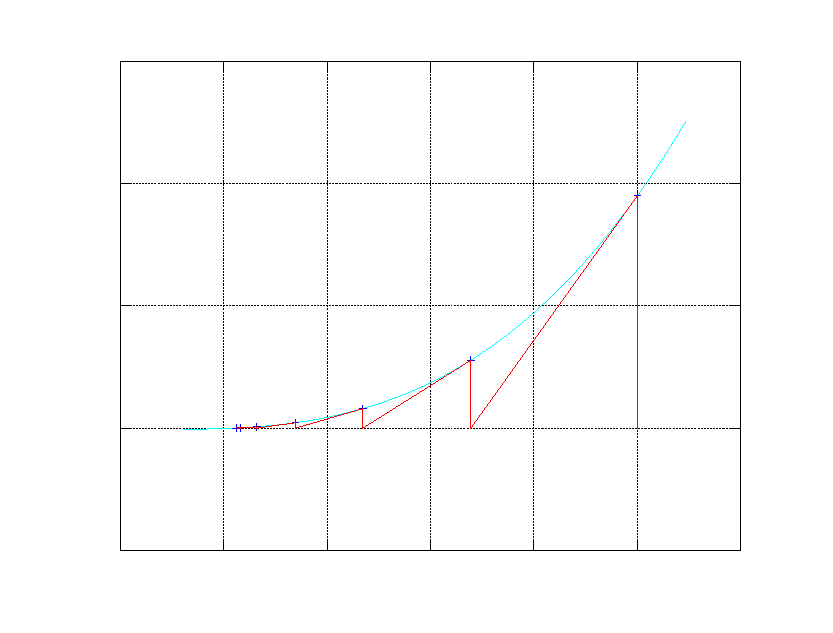
\includegraphics{RadiciEquazione/newton/newtonRecursivePlotOutput}}%
    \gplfronttext
  \end{picture}%
\endgroup

\end{center}

Nel secondo caso studio il punto di innesco $x_{0} = 1$:
\begin{lstlisting}
octave:112> [x, i, ascisse] = newtonMethod('functionNewtonRecursion','functionNewtonRecursionDerivative', 1, 5e1, 1e-14, 1e-14)
Il metodo non converge.
x = -1.00000000000000e+00
i =  5.00000000000000e+01
ascisse = [too long to report here]
octave:113> xNoZero = min(ascisse)-1:0.1:max(ascisse)+1
octave:114> yNoZero = invokeDelegate('functionNewtonRecursion', xNoZero)
octave:115> [prepX, prepY] = prepareForPlottingMethodSegments(ascisse, 'invokeDelegate', 'functionNewtonRecursion')
octave:116> plot(xNoZero, yNoZero, "c", ascisse,invokeDelegate('functionNewtonRecursion', ascisse), "b+", prepX, prepY, "r")
octave:117> grid
octave:118> print 'newtonRecursiveNotConvergencePlotOutput.tex' '-dTex' '-S800,600'
\end{lstlisting}
Il metodo non converge creando una finestra come si vede nel grafico. Questo
l'output del comando \emph{octave:118}:
\begin{center}
% GNUPLOT: LaTeX picture with Postscript
\begingroup
  \makeatletter
  \providecommand\color[2][]{%
    \GenericError{(gnuplot) \space\space\space\@spaces}{%
      Package color not loaded in conjunction with
      terminal option `colourtext'%
    }{See the gnuplot documentation for explanation.%
    }{Either use 'blacktext' in gnuplot or load the package
      color.sty in LaTeX.}%
    \renewcommand\color[2][]{}%
  }%
  \providecommand\includegraphics[2][]{%
    \GenericError{(gnuplot) \space\space\space\@spaces}{%
      Package graphicx or graphics not loaded%
    }{See the gnuplot documentation for explanation.%
    }{The gnuplot epslatex terminal needs graphicx.sty or graphics.sty.}%
    \renewcommand\includegraphics[2][]{}%
  }%
  \providecommand\rotatebox[2]{#2}%
  \@ifundefined{ifGPcolor}{%
    \newif\ifGPcolor
    \GPcolortrue
  }{}%
  \@ifundefined{ifGPblacktext}{%
    \newif\ifGPblacktext
    \GPblacktexttrue
  }{}%
  % define a \g@addto@macro without @ in the name:
  \let\gplgaddtomacro\g@addto@macro
  % define empty templates for all commands taking text:
  \gdef\gplbacktext{}%
  \gdef\gplfronttext{}%
  \makeatother
  \ifGPblacktext
    % no textcolor at all
    \def\colorrgb#1{}%
    \def\colorgray#1{}%
  \else
    % gray or color?
    \ifGPcolor
      \def\colorrgb#1{\color[rgb]{#1}}%
      \def\colorgray#1{\color[gray]{#1}}%
      \expandafter\def\csname LTw\endcsname{\color{white}}%
      \expandafter\def\csname LTb\endcsname{\color{black}}%
      \expandafter\def\csname LTa\endcsname{\color{black}}%
      \expandafter\def\csname LT0\endcsname{\color[rgb]{1,0,0}}%
      \expandafter\def\csname LT1\endcsname{\color[rgb]{0,1,0}}%
      \expandafter\def\csname LT2\endcsname{\color[rgb]{0,0,1}}%
      \expandafter\def\csname LT3\endcsname{\color[rgb]{1,0,1}}%
      \expandafter\def\csname LT4\endcsname{\color[rgb]{0,1,1}}%
      \expandafter\def\csname LT5\endcsname{\color[rgb]{1,1,0}}%
      \expandafter\def\csname LT6\endcsname{\color[rgb]{0,0,0}}%
      \expandafter\def\csname LT7\endcsname{\color[rgb]{1,0.3,0}}%
      \expandafter\def\csname LT8\endcsname{\color[rgb]{0.5,0.5,0.5}}%
    \else
      % gray
      \def\colorrgb#1{\color{black}}%
      \def\colorgray#1{\color[gray]{#1}}%
      \expandafter\def\csname LTw\endcsname{\color{white}}%
      \expandafter\def\csname LTb\endcsname{\color{black}}%
      \expandafter\def\csname LTa\endcsname{\color{black}}%
      \expandafter\def\csname LT0\endcsname{\color{black}}%
      \expandafter\def\csname LT1\endcsname{\color{black}}%
      \expandafter\def\csname LT2\endcsname{\color{black}}%
      \expandafter\def\csname LT3\endcsname{\color{black}}%
      \expandafter\def\csname LT4\endcsname{\color{black}}%
      \expandafter\def\csname LT5\endcsname{\color{black}}%
      \expandafter\def\csname LT6\endcsname{\color{black}}%
      \expandafter\def\csname LT7\endcsname{\color{black}}%
      \expandafter\def\csname LT8\endcsname{\color{black}}%
    \fi
  \fi
  \setlength{\unitlength}{0.0500bp}%
  \begin{picture}(7680.00,5760.00)%
    \gplgaddtomacro\gplbacktext{%
      \colorrgb{0.00,0.00,0.00}%
      \put(866,634){\makebox(0,0)[r]{\strut{}-6}}%
      \colorrgb{0.00,0.00,0.00}%
      \put(866,1416){\makebox(0,0)[r]{\strut{}-4}}%
      \colorrgb{0.00,0.00,0.00}%
      \put(866,2198){\makebox(0,0)[r]{\strut{}-2}}%
      \colorrgb{0.00,0.00,0.00}%
      \put(866,2981){\makebox(0,0)[r]{\strut{}0}}%
      \colorrgb{0.00,0.00,0.00}%
      \put(866,3763){\makebox(0,0)[r]{\strut{}2}}%
      \colorrgb{0.00,0.00,0.00}%
      \put(866,4545){\makebox(0,0)[r]{\strut{}4}}%
      \colorrgb{0.00,0.00,0.00}%
      \put(866,5327){\makebox(0,0)[r]{\strut{}6}}%
      \colorrgb{0.00,0.00,0.00}%
      \put(998,414){\makebox(0,0){\strut{}-2}}%
      \colorrgb{0.00,0.00,0.00}%
      \put(1742,414){\makebox(0,0){\strut{}-1.5}}%
      \colorrgb{0.00,0.00,0.00}%
      \put(2486,414){\makebox(0,0){\strut{}-1}}%
      \colorrgb{0.00,0.00,0.00}%
      \put(3230,414){\makebox(0,0){\strut{}-0.5}}%
      \colorrgb{0.00,0.00,0.00}%
      \put(3974,414){\makebox(0,0){\strut{}0}}%
      \colorrgb{0.00,0.00,0.00}%
      \put(4718,414){\makebox(0,0){\strut{}0.5}}%
      \colorrgb{0.00,0.00,0.00}%
      \put(5462,414){\makebox(0,0){\strut{}1}}%
      \colorrgb{0.00,0.00,0.00}%
      \put(6206,414){\makebox(0,0){\strut{}1.5}}%
      \colorrgb{0.00,0.00,0.00}%
      \put(6950,414){\makebox(0,0){\strut{}2}}%
    }%
    \gplgaddtomacro\gplfronttext{%
    }%
    \gplbacktext
    \put(0,0){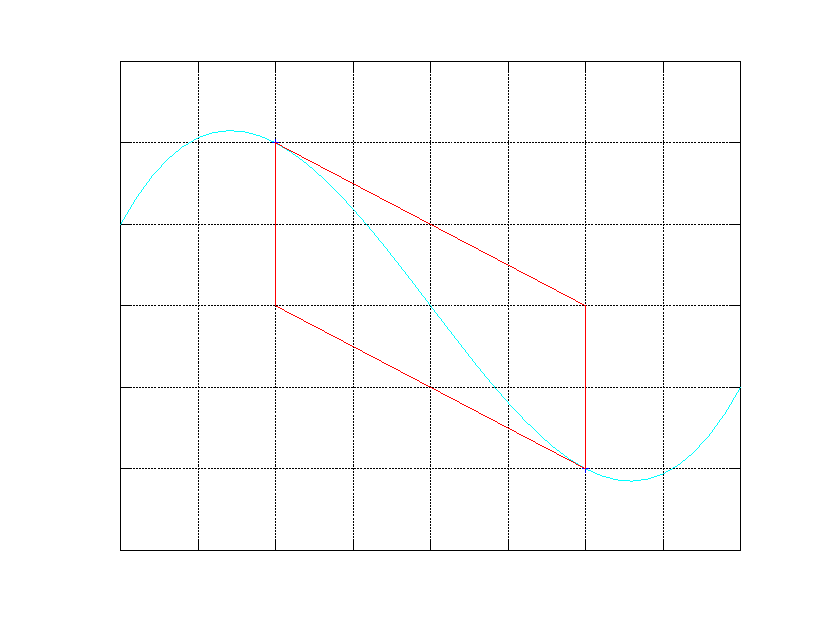
\includegraphics{RadiciEquazione/newton/newtonRecursiveNotConvergencePlotOutput}}%
    \gplfronttext
  \end{picture}%
\endgroup

\end{center}